\documentclass[a4paper,12pt,twoside,printwatermark=true]{modeloLEA}

%% Some pieces required from the pandoc template
\providecommand{\tightlist}{%
  \setlength{\itemsep}{0pt}\setlength{\parskip}{0pt}}

% Use the lineno option to display guide line numbers if required.
% Note that the use of elements such as single-column equations
% may affect the guide line number alignment.

\usepackage[T1]{fontenc}
\usepackage[utf8]{inputenc}

\definecolor{pinpblue}{HTML}{185FAF}  % imagecolorpicker on blue for new R logo
\definecolor{pnasbluetext}{RGB}{101,0,0} %



\title{Relação Entre Velocidade e Distância de Frenagem para Carros de Passeio}

\author[a,b]{Aluno Consultor 1}
\author[a,b]{Aluno Consultor 2}
\author[c,d]{Consulente}
\author[a,e]{Marcus A. Nunes}

  \affil[a]{Departamento de Estatística - UFRN}
  \affil[b]{Consultor}
  \affil[c]{Outro Departamento - UFRN}
  \affil[d]{Consulente}
  \affil[e]{Orientação}

\setcounter{secnumdepth}{5}

% Please give the surname of the lead author for the running footer
\leadauthor{Author and Author}

% Keywords are not mandatory, but authors are strongly encouraged to provide them. If provided, please include two to five keywords, separated by the pipe symbol, e.g:
 \keywords{  regressão linear |  automobilismo |  segurança  }  

\begin{abstract}
Este trabalho estuda a relação entre a velocidade de carros (mph) e a
distância (pés) que eles levaram para parar completamente. Utilizamos
regressão linear simples para determinar se há relação entre estas duas
variáveis.
\end{abstract}

\dates{This version was compiled on \today}

\pinpfootercontents{YourPackage Vignette}

% pacotes a serem utilizados
\usepackage{amsmath}
\numberwithin{equation}{section}
\numberwithin{figure}{section}
\numberwithin{table}{section}
\usepackage{icomma}
\usepackage{mathtools}
\mathtoolsset{showonlyrefs}

\begin{document}

% Optional adjustment to line up main text (after abstract) of first page with line numbers, when using both lineno and twocolumn options.
% You should only change this length when you've finalised the article contents.
\verticaladjustment{-2pt}

\maketitle
\thispagestyle{firststyle}
\ifthenelse{\boolean{shortarticle}}{\ifthenelse{\boolean{singlecolumn}}{\abscontentformatted}{\abscontent}}{}

% If your first paragraph (i.e. with the \dropcap) contains a list environment (quote, quotation, theorem, definition, enumerate, itemize...), the line after the list may have some extra indentation. If this is the case, add \parshape=0 to the end of the list environment.


\hypertarget{objetivos}{%
\section{Objetivos}\label{objetivos}}

Neste trabalho estamos interessados em verificar que existe alguma
relação entre a velocidade de um carro (em milhas por hora) e a
distância que o carro levou para parar (em pés). A hipótese com a qual
trabalhamos é a de que existe uma relação positiva entre estas
variáveis. Isto é, quanto mais rápido um carro estiver viajando, maior
vai ser a distância necessária para que este carro pare completamente.

Além de verificar se há uma relação entre estas variáveis, desejamos uma
relação capaz de prever o quanto uma variável varia em relação a outra.
Assim, gostaríamos de poder estimar a distância necessária para um carro
parar se soubermos qual a sua velocidade.

\hypertarget{metodologia}{%
\section{Metodologia}\label{metodologia}}

Os dados foram obtidos a partir de 50 carros. As medições foram
realizadas na década de 1920 e disponibilizadas no pacote estatístico
\texttt{R}. Não há informações a respeito dos modelos dos carros
utilizados neste experimento.

Utilizaremos um método estatístico chamado regressão linear a fim de
verificar se há relação entre a distância necessária para um carro parar
completamente e sua velocidade. Este é um método bastante popular, capaz
de descrever com bastante precisão a relação entre as variáveis que nos
interessam.

Sejam \(x_1, x_2, \cdots, x_n\) as observações referentes à velocidade
dos carros em questão. Considere \(y_1, y_2, \cdots, y_n\) as
observações referentes à distância necessária para os carros pararem.
Podemos expressar a dependência entre \(y\) e \(x\) através da equação

\begin{equation}
y_i = \beta_0 + \beta_1x_i + \varepsilon_i,
\end{equation}

\noindent onde \(\beta_0\) e \(\beta_1\) são coeficientes estimados
pelas equações

\begin{align}
\widehat{\beta}_1 &= \frac{\sum_{i=1}^n(x_i-\overline{x})(y_i-\overline{y})}{\sum_{i=1}^n(x_i-\overline{x})^2}  \label{estimadores01} \\
\widehat{\beta}_0 &= \overline{y}-\widehat{\beta}_1\overline{x}  \label{estimadores02}
\end{align}

\noindent As quantidades \(\overline{x}\) e \(\overline{y}\) são,
respectivamente, as médias amostrais de \(x_1, x_2, \cdots, x_n\) e
\(y_1, y_2, \cdots, y_n\). Estas médias amostrais são dadas por

\begin{align}
\overline{x} &= \frac{1}{n}\sum_{i=1}^nx_i \\
\overline{y} &= \frac{1}{n}\sum_{i=1}^ny_i 
\end{align}

Determinamos se o coeficiente \(\beta_1\) é estatisticamente
significante através de um teste \(t\). Sob a hipótese nula, assumimos
que o estimador possui distribuição \(t\) com \(n-1\) graus de
liberdade.

\hypertarget{resultados}{%
\section{Resultados}\label{resultados}}

A fim de verificar visualmente se há algum tipo de relação entre as
variáveis consideradas neste estudo, exibimos o gráfico de dispersão dos
dados na Figura \ref{fig:GraficoDispersao}. Note que é possível perceber
uma forte tendência linear positiva na relação entre estas variáveis.
Quanto maior o valor da velocidade, maior a distância necessária para o
carro parar completamente.

\begin{Shaded}
\begin{Highlighting}[]
\KeywordTok{ggplot}\NormalTok{(cars, }\KeywordTok{aes}\NormalTok{(}\DataTypeTok{x=}\NormalTok{speed, }\DataTypeTok{y=}\NormalTok{dist)) }\OperatorTok{+}
\StringTok{  }\KeywordTok{geom_point}\NormalTok{() }\OperatorTok{+}
\StringTok{  }\KeywordTok{labs}\NormalTok{(}\DataTypeTok{x=}\StringTok{"Velocidade (mph)"}\NormalTok{, }\DataTypeTok{y=}\StringTok{"Distância (pés)"}\NormalTok{)}
\end{Highlighting}
\end{Shaded}

\begin{figure}

{\centering 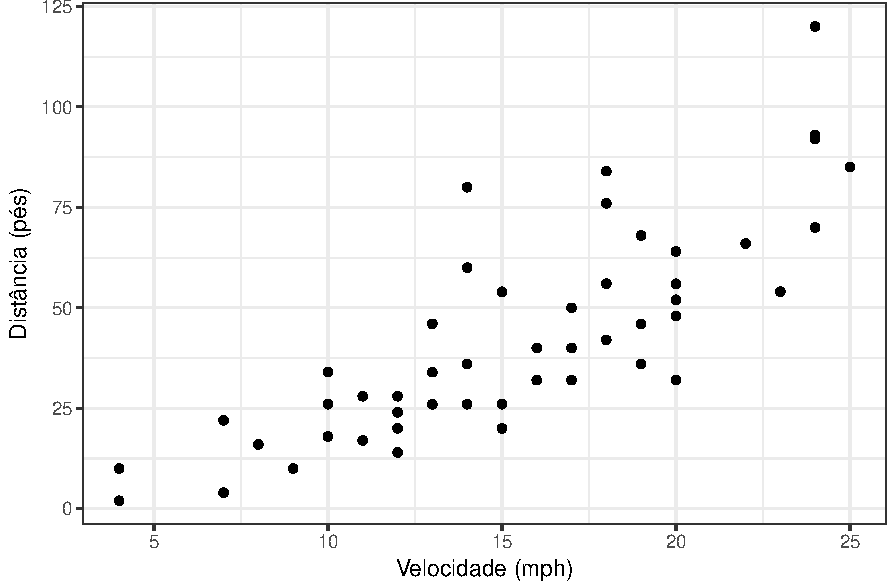
\includegraphics{skeleton_files/figure-latex/GraficoDispersao-1} 

}

\caption{\label{fig:GraficoDispersao} Gráfico de dispersão da distância de parada completa (pés) versus velocidade (mph) dos carros.}\label{fig:GraficoDispersao}
\end{figure}

Além disso, adicionamos ao gráfico exibido na Figura
\ref{fig:GraficoDispersao} a reta que melhor descreve a relação entre
estas variáveis. Esta reta foi obtida através do método descrito na
seção anterior, fazendo uso das fórmulas \eqref{estimadores01} e
\eqref{estimadores02}. Explicitamente, a equação representada na figura
é dada por

\begin{Shaded}
\begin{Highlighting}[]
\NormalTok{ajuste <-}\StringTok{ }\KeywordTok{lm}\NormalTok{(dist }\OperatorTok{~}\StringTok{ }\NormalTok{speed, }\DataTypeTok{data=}\NormalTok{cars)}
\end{Highlighting}
\end{Shaded}

\begin{equation}\label{equacaoFinal}
\widehat{y}_i = -17,5791 + 3,9324x_i.
\end{equation}

Entretanto, precisamos testar se os coeficientes estimados e
apresentados na relação \eqref{equacaoFinal} são, de fato,
estatisticamente significantes. Para isto, testaremos as hipóteses

\begin{align*}
H_0 &: \beta_0 = 0 \\
H_1 &: \beta_0 \neq 0 \\
\end{align*}

\noindent e

\begin{align*}
H_0 &: \beta_1 = 0 \\
H_1 &: \beta_1 \neq 0 \\
\end{align*}

\noindent Os resultados destes testes estão apresentados na Tabela
\ref{tabelaResultados}.

Note que, em ambos os casos, o p-valor encontrado é inferior a
\(\alpha = 0,05\). Portanto, podemos rejeitar ambas as hipóteses nulas e
\(\beta_0\) e \(\beta_1\) são estatisticamente diferentes de zero.

Para finalizar a análise, devemos verificar se o modelo ajustado não
viola as hipóteses do modelo de regressão linear. Para tal, exibimos a
análise de resíduos na Figura \ref{residuos}.

\begin{Shaded}
\begin{Highlighting}[]
\KeywordTok{autoplot}\NormalTok{(ajuste)}
\end{Highlighting}
\end{Shaded}

\begin{center}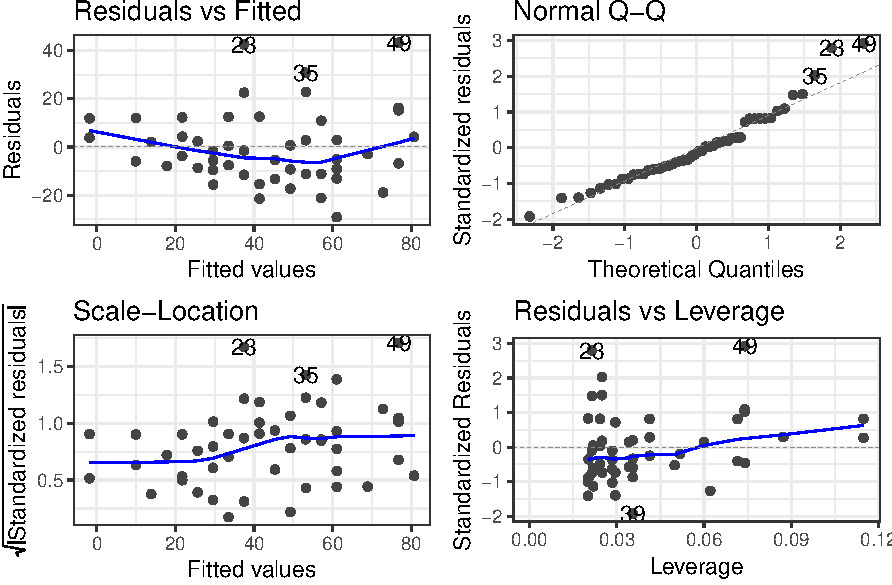
\includegraphics{skeleton_files/figure-latex/residuos-1} \end{center}

Note que na parte superior esquerda da imagem, embora o gráfico dos
resíduos versus valores ajustados não apresente tendência, a variância
não é constante. Note que os pontos próximos de zero estão mais próximos
entre si do que os pontos mais à direita no gráfico. Portanto, há uma
violação das hipóteses da regressão linear neste caso.

Assim, podemos sugerir uma transformação nestes dados ou a utilização de
outro método de análise, como um modelo linear generalizado.

%\showmatmethods


\bibliography{modeloLEA}
\bibliographystyle{jss}



\end{document}

